\documentclass[handout]{beamer} %

 
\mode<presentation>
{
%\usetheme[titleprogressbar]{m}
  \usetheme{default}      % or try Darmstadt, Madrid, Warsaw, ...
  \usecolortheme{default} % or try albatross, beaver, crane, ...
  \usefonttheme{default}  % or try serif, structurebold, ...
  \setbeamertemplate{navigation symbols}{}
  \setbeamertemplate{caption}[numbered]
} 

\setbeamerfont{section in toc}{size=\Large}
\setbeamerfont{subsection in toc}{size=\large}
\addtobeamertemplate{navigation symbols}{}{%
    \usebeamerfont{footline}%
    \usebeamercolor[fg]{footline}%
    \hspace{1em}%
    \insertframenumber/\inserttotalframenumber
}

\usepackage{scrextend}

\usepackage[english]{babel}
\usepackage{color}
\usepackage[utf8x]{inputenc}
\usepackage{booktabs}
\usepackage{colortbl}
\usepackage{verbatim}
\usepackage{bm}
\usepackage{listings}
\usepackage{amsmath} 
\usepackage{hyperref}
\usepackage{array}
\usepackage{wasysym}
\usepackage{xmpmulti}
\usepackage{url}
\newcommand{\bTheta}{\bm{\Theta}}

%\newcounter{propCounter} 

\newtheorem{prop}{Proposition}
 \setbeamertemplate{theorems}[numbered]


\makeatletter
\renewenvironment{proof}[1][\proofname]{\par
  \pushQED{\qed}%
  \normalfont \topsep6\p@\@plus6\p@\relax
  \trivlist
  \item[\hskip\labelsep
        \itshape
    #1\@addpunct{.}]\mbox{} 
}{%
  \popQED\endtrivlist\@endpefalse
}
 
\newenvironment<>{proofs}[1][\proofname]{%
    \par
    \def\insertproofname{#1\@addpunct{.}}%
    \usebeamertemplate{proof begin}#2}
  {\usebeamertemplate{proof end}}
 \newenvironment<>{proofe}{%
    \par
    \pushQED{\qed}
    \setbeamertemplate{proof begin}{\begin{block}{}}
    \usebeamertemplate{proof begin}}
  {\popQED\usebeamertemplate{proof end}}

\makeatother




\def\blockSqz{\vspace*{-\baselineskip}\setlength\belowdisplayshortskip{0pt}}
\def\Put(#1,#2)#3{\leavevmode\makebox(0,0){\put(#1,#2){#3}}}
\usepackage{mathtools}
\hypersetup{colorlinks=false,linkcolor=green,pdfborderstyle={/S/U/W 1}}
\usepackage{tikz}
\def\checkmark{\tikz\fill[scale=0.4](0,.35) -- (.25,0) -- (1,.7) -- (.25,.15) -- cycle;} 
\usetikzlibrary{decorations.pathreplacing,calc}

\newcommand{\tikzmark}[2][-3pt]{\tikz[remember picture, overlay, baseline=-0.5ex]\node[#1](#2){};}

\tikzset{brace/.style={decorate, decoration={brace}},
 brace mirrored/.style={decorate, decoration={brace,mirror}},
}

\newcounter{brace}
\setcounter{brace}{0}
\newcommand{\drawbrace}[3][brace]{%
 \refstepcounter{brace}
 \tikz[remember picture, overlay]\draw[#1] (#2.center)--(#3.center)node[pos=0.5, name=brace-\thebrace]{};
}

\newcounter{arrow}
\setcounter{arrow}{0}
\newcommand{\drawcurvedarrow}[3][]{%
 \refstepcounter{arrow}
 \tikz[remember picture, overlay]\draw (#2.center)edge[#1]node[coordinate,pos=0.5, name=arrow-\thearrow]{}(#3.center);
}

% #1 options, #2 position, #3 text 
\newcommand{\annote}[3][]{%
 \tikz[remember picture, overlay]\node[#1] at (#2) {#3};
}
\usepackage{ellipsis} \renewcommand{\ellipsisgap}{0.05em}
\lstset{ 
  basicstyle=\ttfamily\footnotesize
}
\def\a{\alpha}
\def\dash{\text{ --- }}
\def\E{\mathbb{E}}
\def\one{\mathbf{1}}
\def\xit[#1]{{(x^{({#1})})}^T}%{(x^{(1)})}^T }
\DeclareMathOperator*{\argmin}{arg\!\min}
\DeclareMathOperator*{\argmax}{\arg\!\max} 
\usepackage{color} 
\usepackage{listings} 
\usepackage{setspace} 

\definecolor{Code}{rgb}{0,0,0} 
\definecolor{Decorators}{rgb}{0.5,0.5,0.5} 
\definecolor{Numbers}{rgb}{0.5,0,0} 
\definecolor{MatchingBrackets}{rgb}{0.25,0.5,0.5} 
\definecolor{Keywords}{rgb}{0,0,1} 
\definecolor{self}{rgb}{0,0,0} 
\definecolor{Strings}{rgb}{0,0.63,0} 
\definecolor{Comments}{rgb}{0,0.63,1} 
\definecolor{Backquotes}{rgb}{0,0,0} 
\definecolor{Classname}{rgb}{0,0,0} 
\definecolor{FunctionName}{rgb}{0,0,0} 
\definecolor{Operators}{rgb}{0,0,0} 
\definecolor{Background}{rgb}{0.98,0.98,0.98} 
 
\lstdefinelanguage{Python}{ 
numbers=left, 
numberstyle=\footnotesize, 
numbersep=1em, 
xleftmargin=1em, 
framextopmargin=2em, 
framexbottommargin=2em, 
showspaces=false, 
showtabs=false, 
showstringspaces=false, 
frame=l, 
tabsize=4, 
% Basic 
basicstyle=\ttfamily\small\setstretch{1}, 
backgroundcolor=\color{Background}, 
% Comments 
commentstyle=\color{Comments}\slshape, 
% Strings 
stringstyle=\color{Strings}, 
morecomment=[s][\color{Strings}]{"""}{"""}, 
morecomment=[s][\color{Strings}]{'''}{'''}, 
% keywords 
morekeywords={import,from,class,def,for,while,if,is,in,elif,else,not,and,or,print,break,continue,return,True,False,None,access,as,,del,except,exec,finally,global,import,lambda,pass,print,raise,try,assert}, 
keywordstyle={\color{Keywords}\bfseries}, 
% additional keywords 
morekeywords={[2]@invariant,pylab,numpy,np,scipy}, 
keywordstyle={[2]\color{Decorators}\slshape}, 
emph={self}, 
emphstyle={\color{self}\slshape}, 
% 
} 
\title[Learning From Data]{Lfdnn \\ A neural network library for tutorial purpose}

%\author{Shao-Lun Huang  \quad shaolun.huang@sz.tsinghua.edu.cn  }%\\
 %\smallskip
\author{ Feng Zhao  \\ GitHub ID: zhaofeng-shu33}
%\institute{TBSI}
\date{11/22/2020}

\begin{document}
\setbeamertemplate{caption}{\raggedright\insertcaption\par}
\newcommand{\myalert}[1][]{\color{red} #1}
\begin{frame}
  \titlepage
\end{frame}


\AtBeginSection[]{%
  \begin{frame}<beamer> 
  
  \tableofcontents[ 
    currentsubsection, 
    hideothersubsections, 
    sectionstyle=show/hide, 
    subsectionstyle=show/shaded/hide]
  \end{frame}
  \addtocounter{framenumber}{-1}% If you don't want them to affect the slide number
}
 % Uncomment these lines for an automatically generated outline.
 %\begin{frame}{Outline}
 % \tableofcontents
 %\end{frame}
 
\begin{frame}
\tableofcontents
\end{frame}
 
\begin{frame}{Overview}

%\begin{enumerate}
 %\item 
 
 \begin{itemize}
 % \item Review on Generalized Linear Models
 \item neural network and libraries
  \item Autodiff and multilayer neural network
  \begin{itemize}
  	\item Terminology and API
  	\item Implementation detail
  	\item Examples
  \end{itemize}
  \item Practical guide
  \end{itemize}  
\end{frame}
\section{Artificial neural network as homework}
\begin{frame}
\frametitle{Artificial neural network}

\begin{columns}
	\column{0.5\textwidth}
	
	\begin{figure}[!ht]
		\centering
		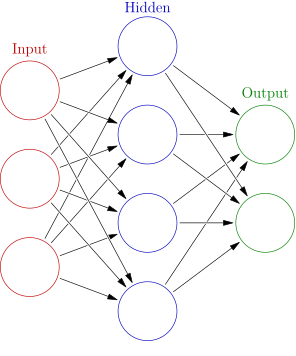
\includegraphics[width=4cm]{nn.png}
		\caption{Three-layered neural network}
	\end{figure}
	\column{0.5\textwidth}

\begin{itemize}
	\item Industrial libraries: for real-world applications
	\item \textbf{Toy libraries}: for understanding the principles of NN
\end{itemize}

\end{columns}
\end{frame}
\begin{frame}
\frametitle{Principles of neural network}
Multilayer perceptron
\begin{align*}
h_0 &= x \\
h_i &= \sigma(w_i \cdot h_{i-1} + b_i), i = 1, \dots, k \\
\hat{y} &= \textrm{softmax}(w \cdot h_k + b)
\end{align*}
with loss function
\begin{align*}
\ell(w, b)
= \sum_{i=1}^{m} \textrm{cross\_entropy}(y_i, \hat{y}_i)
\end{align*}

Use stochastic gradient descent to minimize $\ell(w, b)$:
\begin{equation*}
\ell(w, b)_{t+1} \leftarrow \ell(w, b)_t - \alpha \nabla \ell(w, b)_t
\end{equation*}
$\alpha: $ learning rate

\end{frame}
\begin{frame}{Implementing Neural Network as Homework}
\begin{itemize}
\item Multi-class classifier on CIFAR10 datasets
\vskip0.5em
\begin{minipage}{0.9\textwidth}
	\color{gray}
Try to implement a simple fully-connected neural network and back propagation by yourself.
You are required to complete the Q4: Two-Layer Neural Networkin  Stanford cs231n 2016 winter assignment1.
The original description can be found at \url{http://cs231n.github.io/assignments2016/assignment1/}. 
\end{minipage}
% https://cs231n.github.io/assignments2016/assignment1/
% https://github.com/zhaofeng-shu33/machine_learning_coursework/blob/master/a4/cs231n/classifiers/neural_net.py
% https://github.com/zhaofeng-shu33/neural_net_basic/blob/master/neural_net_cross_entropy.py
\item Function approximation
\begin{minipage}{0.9\textwidth}
	\color{gray}
	Suppose we are given a dataset $\{x^{(i)},y^{(i)}: i=1,2,...,m \}$ generated by
	\begin{equation}
	y^{(i)} = \sin x^{(i)} \quad \forall i
	\end{equation}
	Please design a neural network to represent this function using back-propagation.
\end{minipage}
\item Auto-encoder, xor dataset, mnist dataset etc.
%\item Lfdnn (This semester)
\end{itemize}
\end{frame}
\section{Learning from data neural network}
\begin{frame}
\textit{Learning from data}, a graduate course of Tsinghua Berkeley Shenzhen Institute

\begin{block}{Programming Assignment 2}
\begin{itemize}
	\item Implement \textit{tensor} object
	\item Use the tensor to build a multi-layer classifier model
	\item Build a logistic regression and linear regression model
\end{itemize}
\begin{figure}
	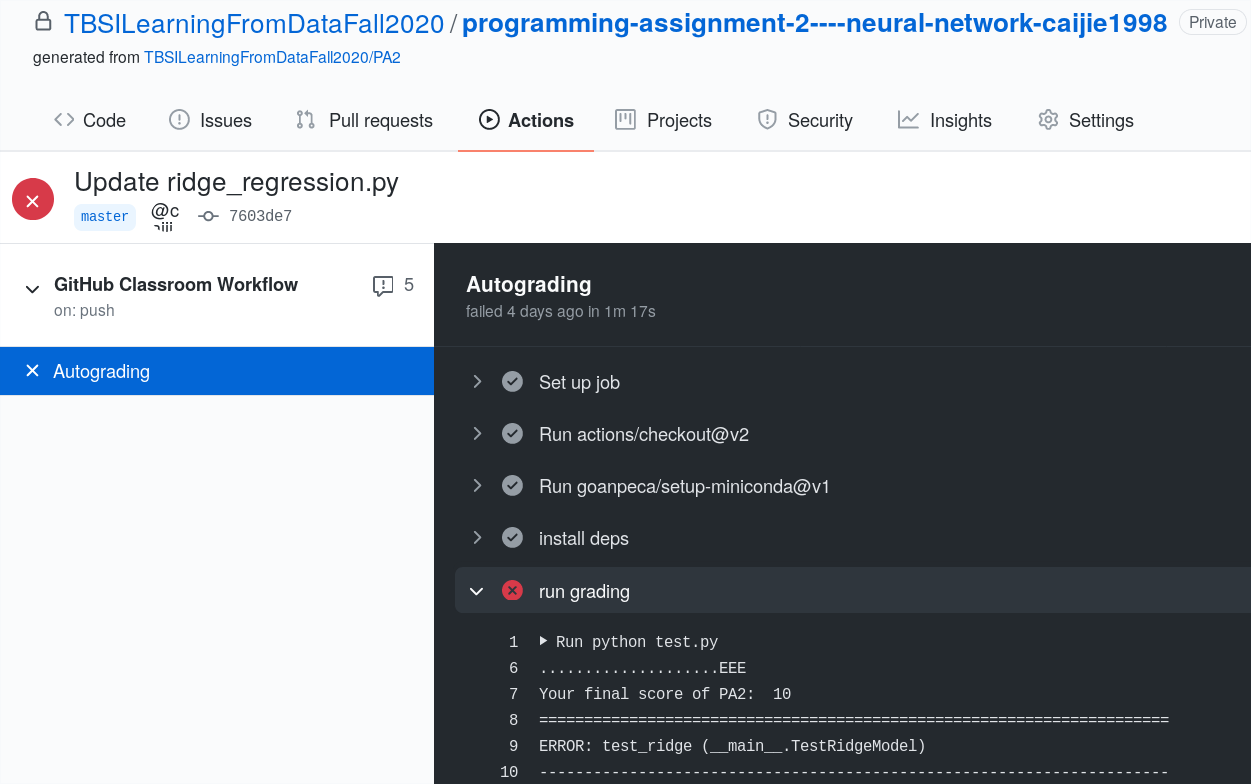
\includegraphics[width=4cm]{auto-grading.png}
\end{figure}
\end{block}
\end{frame}
\begin{frame}[fragile]{Rank 2 tensor}
\begin{itemize}
	\item another name for matrix
	\item vector and scalar: special rank 2 tensor
	\item shape method
\end{itemize}
\begin{lstlisting}[language=Python]
from lfdnn import tensor, operator
a = tensor([3, 4], 't')
print(a.shape)
\end{lstlisting}
\begin{itemize}
	\item concatenation by \textsf{operator}
	\item delayed evaluation
\end{itemize}
\begin{lstlisting}[language=Python,firstnumber=4]
import numpy as np
b = operator.relu(a)
feed = {'t': np.random.normal(size=[3, 4])}
print(b.eval(feed))
\end{lstlisting}
\end{frame}
\section{ Autodiff and multilayer neural network }
\begin{frame}[fragile]{Autodiff and multilayer neural network}
\begin{itemize}
	\item Autodiff: Automatic differentiation
	\item small $h$: $\frac{f(x+h) - f(x)}{h}$ 
	\item use chain rule
\end{itemize}
\begin{lstlisting}[language=Python,firstnumber=8]
print(b.differentiate(a, feed))
print(a.back(b, feed))
\end{lstlisting}
\begin{itemize}
	\item forward pass: \texttt{b.eval}
	\item backward pass: \texttt{b.back}
\end{itemize}
\textbf{Logistic model}
\begin{lstlisting}[language=Python,firstnumber=10]
w = tensor([4, 1], 'w')
b = tensor([1, 1], 'b')
h = operator.add(operator.matmul(a, w), b)
y = operator.sigmoid(h)
feed.update({'w': np.ones([4, 1]),
             'b': np.array([[2]])})
y.eval(feed)
\end{lstlisting}

\end{frame}
\begin{frame}[fragile]{Implementation details}
$f(a) = a^2 + 3a$
\begin{figure}[!ht]
	\centering
	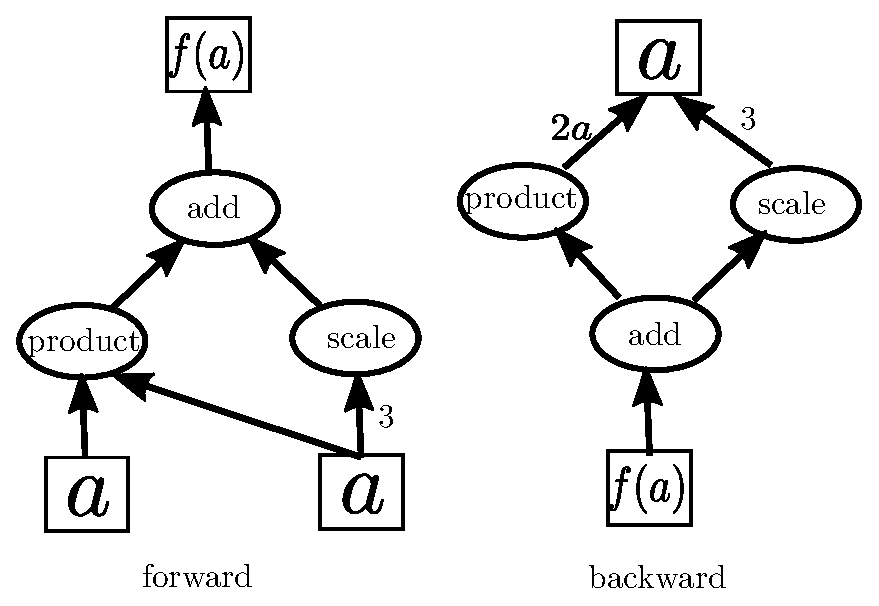
\includegraphics[width=6cm]{auto.eps}
\end{figure}
\begin{lstlisting}[language=Python]
from lfdnn import tensor
class add(tensor):
    def _eval(self, feed):
        pass
    def _derivative(self, feed, input, target):
        pass
\end{lstlisting}

\end{frame}
\begin{frame}[fragile]{Examples}
Implement matrix multiplication \texttt{matmul(A,B)}
\begin{itemize}
	\item \texttt{A = self.input\_list[0]}
	\item \texttt{B = self.input\_list[1]}
\end{itemize}
\begin{lstlisting}[language=Python,numbers=none]
def _eval(self, feed):
    return A @ B
\end{lstlisting}
Suppose \texttt{A} $\neq$ \texttt{B}, using chain rule:
$\frac{\partial f(A \cdot B)}{\partial A} = \nabla_{AB}f \cdot B^{\mathrm{T}}$

\begin{lstlisting}[language=Python,numbers=none]
def _derivative(self, feed, A, target):
    b = self.back(target, feed)
    return b @ B.T
\end{lstlisting}

\end{frame} 
\begin{frame}[fragile]{Practical guide}
\begin{itemize}
	\item cache the computed value to speed up: \texttt{pring(feed)}
\end{itemize}
\end{frame}

\end{document}
